% Homework template for Learning from Data
% by Xiangxiang Xu <xiangxiangxu.thu@gmail.com>
% LAST UPDATE: October 8, 2018
\documentclass[a4paper]{article}
\usepackage[T1]{fontenc}
\usepackage{amsmath, amssymb, amsthm}
% amsmath: equation*, amssymb: mathbb, amsthm: proof
\usepackage{moreenum}
\usepackage{mathtools}
\usepackage{url}
\usepackage{enumitem}
\usepackage{bm}
\usepackage{graphicx}
\usepackage{subcaption}
\usepackage{booktabs} % toprule
\usepackage[mathcal]{eucal}
\usepackage{dsfont}
\usepackage[numbered,framed]{matlab-prettifier}
%% Definitions for Learning from Data
%% UPDATE: October 8, 2018 by Xiangxiang 
\newcommand{\theterm}{Fall 2019}

\newcommand{\thecoursename}{
Tsinghua-Berkeley Shenzhen Institute\\
%\vspace*{0.1in}
\textsc{Learning from Data}
}

\newcommand{\courseheader}{
\vspace*{-1in}
\begin{center}
\thecoursename \\
\theterm
\vspace*{0.1in}
\hrule
\end{center}
}
\newcommand{\uc}{\underline{c}}    % c, vec
\newcommand{\uv}{\underline{v}}    % x, vec
\newcommand{\uw}{\underline{w}}    % w, vec
\newcommand{\ux}{\underline{x}}    % x, vec
\newcommand{\uy}{\underline{y}}    % y, vec
\newcommand{\uz}{\underline{z}}    % z, vec
\newcommand{\um}{\underline{m}}    % m, vec
\newcommand{\ut}{\underline{t}}    % t, vec
\newcommand{\bc}{\bm{c}}    % c, vec
\newcommand{\bv}{\bm{v}}    % x, vec
\newcommand{\bw}{\bm{w}}    % w, vec
\newcommand{\bx}{\bm{x}}    % x, vec
\newcommand{\by}{\bm{y}}    % y, vec
\newcommand{\bz}{\bm{z}}    % z, vec
% \newcommand{\bm}{\bm{m}}    % m, vec
\newcommand{\bt}{\bm{t}}    % t, vec

\newcommand{\balpha}{\bm{\alpha}}    % alpha, vec
\newcommand{\bxi}{\bm{\xi}}    % xi, vec


\newcommand{\rvx}{\mathsf{x}}    % x, r.v.
\newcommand{\rvy}{\mathsf{y}}    % y, r.v.
\newcommand{\rvz}{\mathsf{z}}    % z, r.v.
\newcommand{\rvw}{\mathsf{w}}    % w, r.v.
\newcommand{\rvv}{\mathsf{v}}    % v, r.v.
\newcommand{\rvm}{\mathsf{m}}    % m, r.v.
\newcommand{\rvt}{\mathsf{t}}    % t, r.v.
\newcommand{\rvH}{\mathsf{H}}    % H, r.v.
\newcommand{\urvx}{\underline{\mathsf{x}}}    % x, r.v. vec
\newcommand{\urvy}{\underline{\mathsf{y}}}    % y, r.v. vec
\newcommand{\urvz}{\underline{\mathsf{z}}}    % z, r.v. vec
\newcommand{\urvw}{\underline{\mathsf{w}}}    % w, r.v. vec
\newcommand{\urvt}{\underline{\mathsf{t}}}    % t, r.v. vec
\newcommand{\defeq}{\triangleq} %\coloneqq
\newcommand{\reals}{\mathbb{R}}
\newcommand{\T}{\mathrm{T}}    % transpose
\newcommand{\BLS}{\mathrm{BLS}}    % BLS
\newcommand{\LLS}{\mathrm{LLS}}    % LLS
\newcommand{\MVU}{\mathrm{MVU}}    % MVU

\DeclareMathOperator*{\maximize}{maximize}    % maximize
\DeclareMathOperator*{\minimize}{minimize}    % minimize
\newcommand{\st}{\mathrm{subject~to}}    % minimize


% \newcommand{\E}[1]{\mathbb{E}\left[{#1}\right]}
% \newcommand{\Prob}[1]{\mathbb{P}\left({#1}\right)}
\DeclareMathOperator*{\argmax}{arg\,max}
\DeclareMathOperator*{\argmin}{arg\,min}
\DeclareMathOperator*{\argsup}{arg\,sup}
\DeclareMathOperator*{\arginf}{arg\,inf}
\DeclareMathOperator{\Var}{Var}
\DeclareMathOperator{\Cov}{Cov}
\DeclareMathOperator{\MSE}{MSE}
\DeclareMathOperator{\1}{\mathds{1}}
\DeclareMathOperator{\E}{\mathbb{E}}
\DeclareMathOperator{\Prob}{\mathbb{P}}

\newcommand\independent{\protect\mathpalette{\protect\independenT}{\perp}}
\def\independenT#1#2{\mathrel{\rlap{$#1#2$}\mkern2mu{#1#2}}}


\lstset{
  style              = Matlab-editor,
  captionpos         =b,
  basicstyle         = \mlttfamily,
  escapechar         = ",
  mlshowsectionrules = true,
}
\begin{document}
\courseheader



\newcounter{hwcnt}
\setcounter{hwcnt}{4} % set to the times of Homework

\begin{center}
  \underline{\bf Programming Homework 4}%\thehwcnt} \\
\end{center}
\begin{flushleft}
  TIAN Chenyu\hfill
  \today
\end{flushleft}
\hrule

\vspace{2em}
\setlist[enumerate,1]{label=\thehwcnt.\arabic*.}
\setlist[enumerate,2]{label=(\alph*)}
\setlist[enumerate,3]{label=\roman*.}
\setlist[enumerate,4]{label=\greek*)}

\flushleft
\rule{\textwidth}{1pt}
\begin{itemize}
\item {\bf Acknowledgments: \/} 
  This template takes some materials from course CSE 547/Stat 548 of Washington University: \small{\url{https://courses.cs.washington.edu/courses/cse547/17sp/index.html}}.
\item {\bf Collaborators: \/}
  I finish this homework by myself.
  % \begin{itemize}
  % \item 1.2 (b) was solved with the help from \underline{\hspace{3em}}.
  % \item Discussion with \underline{\hspace{3em}} helped me finishing 1.3.
  % \end{itemize}
\end{itemize}
\rule{\textwidth}{1pt}

\vspace{2em}

% You may use \texttt{enumerate} to generate answers for each question:

% 4.2
\begin{enumerate}
  \setlength{\itemsep}{4\parskip}
  \item The code is in the \emph{Q\_learning.py}.
  \item 
  The matrix of learned reward is shown in \ref{fig:1}. The MSE is 0.08.
  \begin{figure}[htbp]
    \centering
    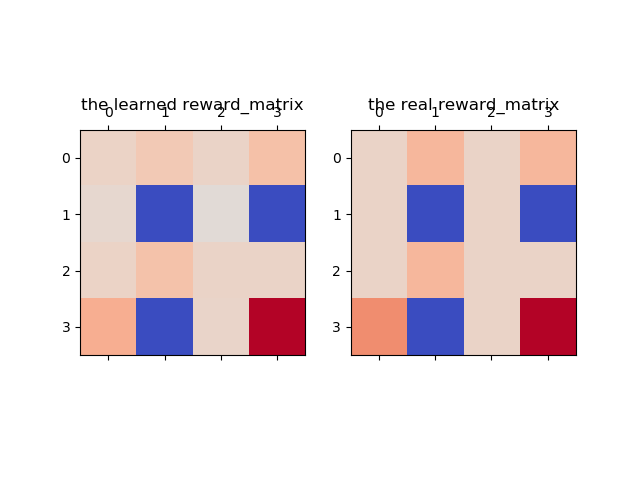
\includegraphics[width = 0.8\textwidth]{../distribution.png}
    \caption{Matrix Distribution}
    \label{fig:1}
  \end{figure}
  \newline The most different part is (3, 0), where the reward is 2 but the learned reward is 1.23.
  \newline Explanation: It is obvious that (3, 0) is near the trap. In the beginning, because of random action, the mouse is easy to get a negative reward if starts from here.
  As the $\epsilon$ getting smaller afterwards, then (3,0) is rarely visited for a low Q\_value. 
  Therefore, small samples of Q\_value in (3, 0) leads to some estimation bias.
\newpage

% 4.2
  \item I used Keras 2.3.0 to build the neural network by adding methods in the origin \emph{Agent} class. 
  At each iteration of DQN, a mini-batch of states, actions, rewards, and next states are sampled from the replay memory as observations to train the Q-network, which approximates the Q function.
  \lstinputlisting[firstline=109,lastline=122, firstnumber=0]{../dqn_10_10.py}
  
  \begin{figure}
    \begin{subfigure}[H]{0.5\textwidth}
      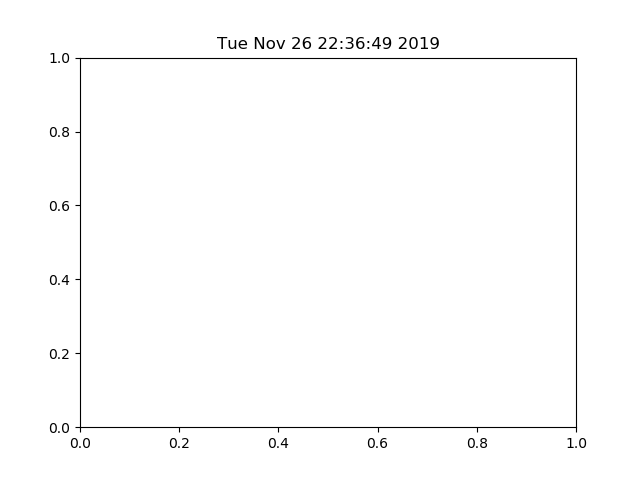
\includegraphics[width=\textwidth]{../10_10_dqn.png}
      \caption{The Learned route by DQN}
      \label{fig:2}
    \end{subfigure}
    %
    \begin{subfigure}[H]{0.5\textwidth}
      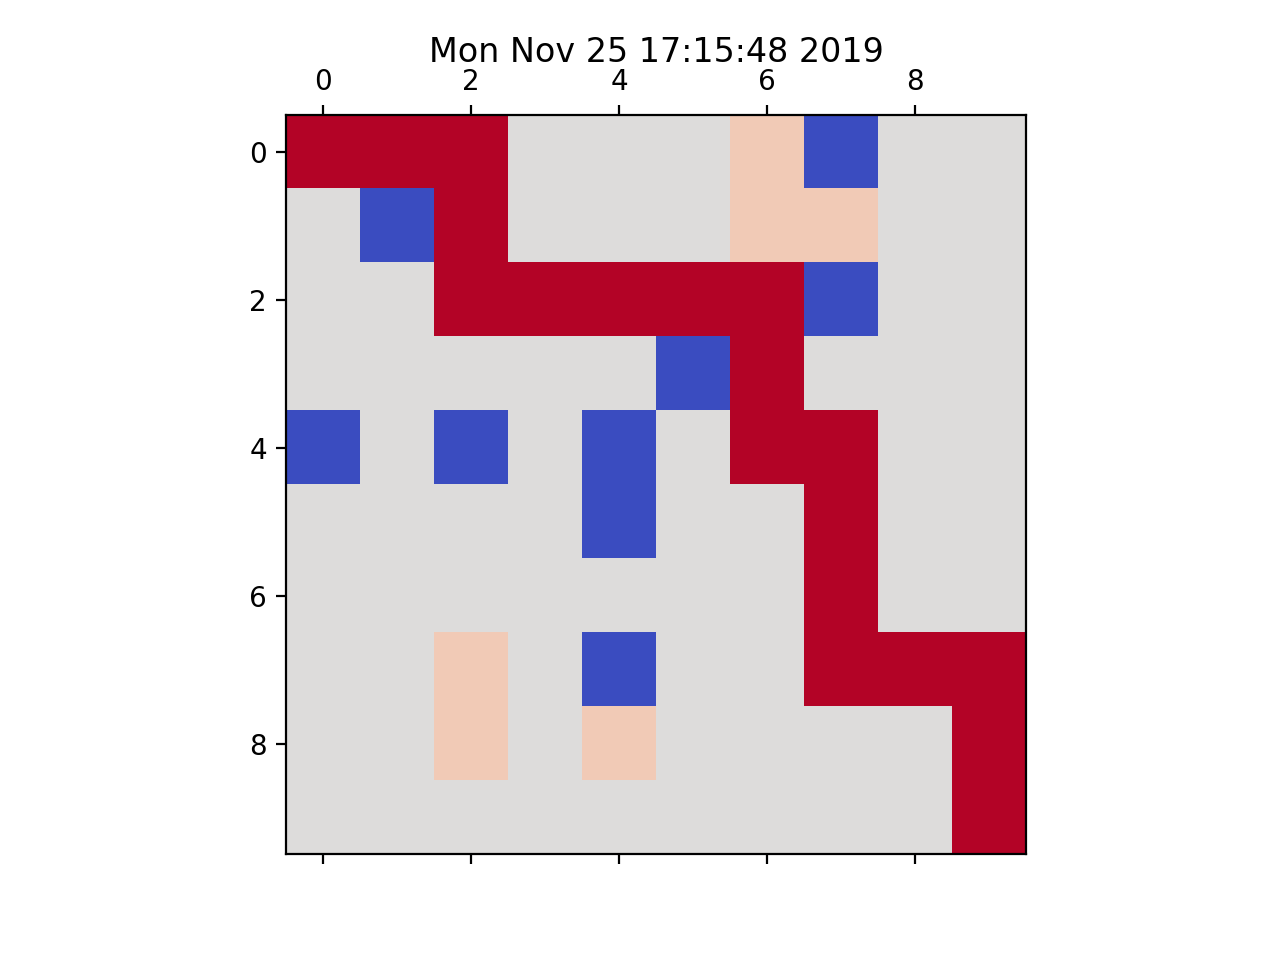
\includegraphics[width=\textwidth]{../10_10_q_table.png}
      \caption{The Learned route by Q-table}
      \label{fig:3}
    \end{subfigure}
  \end{figure}
  DQN works and finds some different routes from the Q\_table method as shown in the \ref{fig:2}.
  \newline There are some comparisons between 2 methods:
  \begin{enumerate}
    \item In this 10*10 senario, DQN takes much more time to train the agent than q-table. 
    \item It is more difficult to tune the DQN hyperparameters such as netword architecture and batch size. But Q\_table is only have to tune learning rate.
    \item The solution of Q\_table is stable. But the learned solution of DQN can be different everytime.
    \item The DQN learned actions sometimes can fall into dead loop. For example, its action can be go left then go right, repeat this pair of actions forever. So the maximum steps need to be set to jump out of the loop.
    \item In this discrete senario, I think Q learning is more efficient. But DQN is more flexible to complex tasks with continous states and actions.
  \end{enumerate}

  The source code could be found in \emph{dqn\_10\_10.py}. Here are the core codes:
  \lstinputlisting[firstline=188,lastline=209, firstnumber=0]{../dqn_10_10.py}
\end{enumerate}
  
  % \newpage
  
  % \appendix
  % \section{Source code}
  % \label{sec:a:code}
  % % \lstlistoflistings
  % Source code for plotting Figure \ref{fig:1} is shown as follows.
  % \lstinputlisting{matlabscript.m}
  
\end{document}
%%% Local Variables:
%%% mode: latex
%%% TeX-master: t
%%% End:
